\documentclass[twoside]{book}

% Packages required by doxygen
\usepackage{fixltx2e}
\usepackage{calc}
\usepackage{doxygen}
\usepackage[export]{adjustbox} % also loads graphicx
\usepackage{graphicx}
\usepackage[utf8]{inputenc}
\usepackage{makeidx}
\usepackage{multicol}
\usepackage{multirow}
\PassOptionsToPackage{warn}{textcomp}
\usepackage{textcomp}
\usepackage[nointegrals]{wasysym}
\usepackage[table]{xcolor}

% Font selection
\usepackage[T1]{fontenc}
\usepackage[scaled=.90]{helvet}
\usepackage{courier}
\usepackage{amssymb}
\usepackage{sectsty}
\renewcommand{\familydefault}{\sfdefault}
\allsectionsfont{%
  \fontseries{bc}\selectfont%
  \color{darkgray}%
}
\renewcommand{\DoxyLabelFont}{%
  \fontseries{bc}\selectfont%
  \color{darkgray}%
}
\newcommand{\+}{\discretionary{\mbox{\scriptsize$\hookleftarrow$}}{}{}}

% Page & text layout
\usepackage{geometry}
\geometry{%
  a4paper,%
  top=2.5cm,%
  bottom=2.5cm,%
  left=2.5cm,%
  right=2.5cm%
}
\tolerance=750
\hfuzz=15pt
\hbadness=750
\setlength{\emergencystretch}{15pt}
\setlength{\parindent}{0cm}
\setlength{\parskip}{3ex plus 2ex minus 2ex}
\makeatletter
\renewcommand{\paragraph}{%
  \@startsection{paragraph}{4}{0ex}{-1.0ex}{1.0ex}{%
    \normalfont\normalsize\bfseries\SS@parafont%
  }%
}
\renewcommand{\subparagraph}{%
  \@startsection{subparagraph}{5}{0ex}{-1.0ex}{1.0ex}{%
    \normalfont\normalsize\bfseries\SS@subparafont%
  }%
}
\makeatother

% Headers & footers
\usepackage{fancyhdr}
\pagestyle{fancyplain}
\fancyhead[LE]{\fancyplain{}{\bfseries\thepage}}
\fancyhead[CE]{\fancyplain{}{}}
\fancyhead[RE]{\fancyplain{}{\bfseries\leftmark}}
\fancyhead[LO]{\fancyplain{}{\bfseries\rightmark}}
\fancyhead[CO]{\fancyplain{}{}}
\fancyhead[RO]{\fancyplain{}{\bfseries\thepage}}
\fancyfoot[LE]{\fancyplain{}{}}
\fancyfoot[CE]{\fancyplain{}{}}
\fancyfoot[RE]{\fancyplain{}{\bfseries\scriptsize Generated by Doxygen }}
\fancyfoot[LO]{\fancyplain{}{\bfseries\scriptsize Generated by Doxygen }}
\fancyfoot[CO]{\fancyplain{}{}}
\fancyfoot[RO]{\fancyplain{}{}}
\renewcommand{\footrulewidth}{0.4pt}
\renewcommand{\chaptermark}[1]{%
  \markboth{#1}{}%
}
\renewcommand{\sectionmark}[1]{%
  \markright{\thesection\ #1}%
}

% Indices & bibliography
\usepackage{natbib}
\usepackage[titles]{tocloft}
\setcounter{tocdepth}{3}
\setcounter{secnumdepth}{5}
\makeindex

% Hyperlinks (required, but should be loaded last)
\usepackage{ifpdf}
\ifpdf
  \usepackage[pdftex,pagebackref=true]{hyperref}
\else
  \usepackage[ps2pdf,pagebackref=true]{hyperref}
\fi
\hypersetup{%
  colorlinks=true,%
  linkcolor=blue,%
  citecolor=blue,%
  unicode%
}

% Custom commands
\newcommand{\clearemptydoublepage}{%
  \newpage{\pagestyle{empty}\cleardoublepage}%
}

\usepackage{caption}
\captionsetup{labelsep=space,justification=centering,font={bf},singlelinecheck=off,skip=4pt,position=top}

%===== C O N T E N T S =====

\begin{document}

% Titlepage & ToC
\hypersetup{pageanchor=false,
             bookmarksnumbered=true,
             pdfencoding=unicode
            }
\pagenumbering{roman}
\begin{titlepage}
\vspace*{7cm}
\begin{center}%
{\Large kermit }\\
\vspace*{1cm}
{\large Generated by Doxygen 1.8.11}\\
\end{center}
\end{titlepage}
\clearemptydoublepage
\tableofcontents
\clearemptydoublepage
\pagenumbering{arabic}
\hypersetup{pageanchor=true}

%--- Begin generated contents ---
\chapter{Namespace Index}
\section{Namespace List}
Here is a list of all namespaces with brief descriptions\+:\begin{DoxyCompactList}
\item\contentsline{section}{\hyperlink{namespacekermit}{kermit} }{\pageref{namespacekermit}}{}
\item\contentsline{section}{\hyperlink{namespacekerrlist}{kerrlist} }{\pageref{namespacekerrlist}}{}
\end{DoxyCompactList}

\chapter{Hierarchical Index}
\section{Class Hierarchy}
This inheritance list is sorted roughly, but not completely, alphabetically\+:\begin{DoxyCompactList}
\item \contentsline{section}{kermit.\+Kerr\+G\+UI}{\pageref{classkermit_1_1_kerr_g_u_i}}{}
\item ndarray\begin{DoxyCompactList}
\item \contentsline{section}{kermit.\+Kerr\+Array}{\pageref{classkermit_1_1_kerr_array}}{}
\end{DoxyCompactList}
\item Image\+Collection\begin{DoxyCompactList}
\item \contentsline{section}{kerrlist.\+Kerr\+List}{\pageref{classkerrlist_1_1_kerr_list}}{}
\end{DoxyCompactList}
\end{DoxyCompactList}

\chapter{Class Index}
\section{Class List}
Here are the classes, structs, unions and interfaces with brief descriptions\+:\begin{DoxyCompactList}
\item\contentsline{section}{\hyperlink{classkermit_1_1_kerr_array}{kermit.\+Kerr\+Array} }{\pageref{classkermit_1_1_kerr_array}}{}
\item\contentsline{section}{\hyperlink{classkermit_1_1_kerr_g_u_i}{kermit.\+Kerr\+G\+UI} }{\pageref{classkermit_1_1_kerr_g_u_i}}{}
\item\contentsline{section}{\hyperlink{classkerrlist_1_1_kerr_list}{kerrlist.\+Kerr\+List} }{\pageref{classkerrlist_1_1_kerr_list}}{}
\end{DoxyCompactList}

\chapter{File Index}
\section{File List}
Here is a list of all files with brief descriptions\+:\begin{DoxyCompactList}
\item\contentsline{section}{C\+:/\+Users/phyrct/\+Dropbox/\+Me/\+Coding/kermit/kermit/\hyperlink{kermit_8py}{kermit.\+py} }{\pageref{kermit_8py}}{}
\item\contentsline{section}{C\+:/\+Users/phyrct/\+Dropbox/\+Me/\+Coding/kermit/kermit/\hyperlink{kerrlist_8py}{kerrlist.\+py} }{\pageref{kerrlist_8py}}{}
\end{DoxyCompactList}

\chapter{Namespace Documentation}
\hypertarget{namespacekermit}{}\section{kermit Namespace Reference}
\label{namespacekermit}\index{kermit@{kermit}}
\subsection*{Classes}
\begin{DoxyCompactItemize}
\item 
class \hyperlink{classkermit_1_1_kerr_array}{Kerr\+Array}
\item 
class \hyperlink{classkermit_1_1_kerr_g_u_i}{Kerr\+G\+UI}
\end{DoxyCompactItemize}
\subsection*{Variables}
\begin{DoxyCompactItemize}
\item 
tuple \hyperlink{namespacekermit_a9126e144cfcf0e62c9540ceab41357f6}{G\+R\+A\+Y\+\_\+\+R\+A\+N\+GE} = (0,65535)
\item 
tuple \hyperlink{namespacekermit_a79b097e6dc51ad46c17adc76d122c74e}{I\+M\+\_\+\+S\+I\+ZE} = (512,672)
\item 
tuple \hyperlink{namespacekermit_a3a00797e39aca7adb4a8cbfa3406d08a}{A\+N\+\_\+\+I\+M\+\_\+\+S\+I\+ZE} = (554,672)
\item 
tuple \hyperlink{namespacekermit_aa7fd97127ffdc923b5f393978698c4e2}{String\+Types} = (str,unicode)
\item 
string \hyperlink{namespacekermit_adf8dfb894042e43e52e8c1fb73ee6b5c}{ex\+\_\+data1} = \textquotesingle{}Example\+Data1\textquotesingle{}
\item 
string \hyperlink{namespacekermit_a840f1a32f7048a0fa6a2ccb4d98f52eb}{ex\+\_\+data2} = \textquotesingle{}Example\+Data2\textquotesingle{}
\item 
string \hyperlink{namespacekermit_aecc2d1d7664b16df7d95dcb97870f517}{tmp\+\_\+dir} = \textquotesingle{}tmp\textquotesingle{}
\item 
string \hyperlink{namespacekermit_abbd557f9a28767ae9aca37bb210289f2}{example\+\_\+im\+\_\+fol} = r\textquotesingle{}C\+:\textbackslash{}\+Users\textbackslash{}phyrct\textbackslash{}\+Dropbox\textbackslash{}\+Me\textbackslash{}\+Coding\textbackslash{}kermit\textquotesingle{}
\item 
\hyperlink{namespacekermit_a0744c104c9fe9a76f9518b49a1df33b2}{bkim} = io.\+imread(\textquotesingle{}bknd.\+png\textquotesingle{})
\item 
\hyperlink{namespacekermit_a9fb3ba81b634d3ff357261211ff1c453}{unpim} = io.\+imread(\textquotesingle{}unpro.\+png\textquotesingle{})
\item 
\hyperlink{namespacekermit_ace003936bdb5e0aba435651a827c4293}{im} = io.\+imread(\textquotesingle{}sub.\+png\textquotesingle{})
\item 
list \hyperlink{namespacekermit_a8b94ad1d18d6a20c42cad6d65ed1a781}{proc\+\_\+list} = \mbox{[}\hyperlink{namespacekermit_ace003936bdb5e0aba435651a827c4293}{im}\mbox{]}
\item 
\hyperlink{namespacekermit_afc1e6acdf61366d1c0f44edbc11ff790}{v1} = Collection\+Viewer(\hyperlink{namespacekermit_a8b94ad1d18d6a20c42cad6d65ed1a781}{proc\+\_\+list})
\end{DoxyCompactItemize}


\subsection{Variable Documentation}
\index{kermit@{kermit}!A\+N\+\_\+\+I\+M\+\_\+\+S\+I\+ZE@{A\+N\+\_\+\+I\+M\+\_\+\+S\+I\+ZE}}
\index{A\+N\+\_\+\+I\+M\+\_\+\+S\+I\+ZE@{A\+N\+\_\+\+I\+M\+\_\+\+S\+I\+ZE}!kermit@{kermit}}
\subsubsection[{\texorpdfstring{A\+N\+\_\+\+I\+M\+\_\+\+S\+I\+ZE}{AN_IM_SIZE}}]{\setlength{\rightskip}{0pt plus 5cm}tuple kermit.\+A\+N\+\_\+\+I\+M\+\_\+\+S\+I\+ZE = (554,672)}\hypertarget{namespacekermit_a3a00797e39aca7adb4a8cbfa3406d08a}{}\label{namespacekermit_a3a00797e39aca7adb4a8cbfa3406d08a}
\index{kermit@{kermit}!bkim@{bkim}}
\index{bkim@{bkim}!kermit@{kermit}}
\subsubsection[{\texorpdfstring{bkim}{bkim}}]{\setlength{\rightskip}{0pt plus 5cm}kermit.\+bkim = io.\+imread(\textquotesingle{}bknd.\+png\textquotesingle{})}\hypertarget{namespacekermit_a0744c104c9fe9a76f9518b49a1df33b2}{}\label{namespacekermit_a0744c104c9fe9a76f9518b49a1df33b2}
\index{kermit@{kermit}!ex\+\_\+data1@{ex\+\_\+data1}}
\index{ex\+\_\+data1@{ex\+\_\+data1}!kermit@{kermit}}
\subsubsection[{\texorpdfstring{ex\+\_\+data1}{ex_data1}}]{\setlength{\rightskip}{0pt plus 5cm}string kermit.\+ex\+\_\+data1 = \textquotesingle{}Example\+Data1\textquotesingle{}}\hypertarget{namespacekermit_adf8dfb894042e43e52e8c1fb73ee6b5c}{}\label{namespacekermit_adf8dfb894042e43e52e8c1fb73ee6b5c}
\index{kermit@{kermit}!ex\+\_\+data2@{ex\+\_\+data2}}
\index{ex\+\_\+data2@{ex\+\_\+data2}!kermit@{kermit}}
\subsubsection[{\texorpdfstring{ex\+\_\+data2}{ex_data2}}]{\setlength{\rightskip}{0pt plus 5cm}string kermit.\+ex\+\_\+data2 = \textquotesingle{}Example\+Data2\textquotesingle{}}\hypertarget{namespacekermit_a840f1a32f7048a0fa6a2ccb4d98f52eb}{}\label{namespacekermit_a840f1a32f7048a0fa6a2ccb4d98f52eb}
\index{kermit@{kermit}!example\+\_\+im\+\_\+fol@{example\+\_\+im\+\_\+fol}}
\index{example\+\_\+im\+\_\+fol@{example\+\_\+im\+\_\+fol}!kermit@{kermit}}
\subsubsection[{\texorpdfstring{example\+\_\+im\+\_\+fol}{example_im_fol}}]{\setlength{\rightskip}{0pt plus 5cm}string kermit.\+example\+\_\+im\+\_\+fol = r\textquotesingle{}C\+:\textbackslash{}\+Users\textbackslash{}phyrct\textbackslash{}\+Dropbox\textbackslash{}\+Me\textbackslash{}\+Coding\textbackslash{}kermit\textquotesingle{}}\hypertarget{namespacekermit_abbd557f9a28767ae9aca37bb210289f2}{}\label{namespacekermit_abbd557f9a28767ae9aca37bb210289f2}
\index{kermit@{kermit}!G\+R\+A\+Y\+\_\+\+R\+A\+N\+GE@{G\+R\+A\+Y\+\_\+\+R\+A\+N\+GE}}
\index{G\+R\+A\+Y\+\_\+\+R\+A\+N\+GE@{G\+R\+A\+Y\+\_\+\+R\+A\+N\+GE}!kermit@{kermit}}
\subsubsection[{\texorpdfstring{G\+R\+A\+Y\+\_\+\+R\+A\+N\+GE}{GRAY_RANGE}}]{\setlength{\rightskip}{0pt plus 5cm}tuple kermit.\+G\+R\+A\+Y\+\_\+\+R\+A\+N\+GE = (0,65535)}\hypertarget{namespacekermit_a9126e144cfcf0e62c9540ceab41357f6}{}\label{namespacekermit_a9126e144cfcf0e62c9540ceab41357f6}
\index{kermit@{kermit}!im@{im}}
\index{im@{im}!kermit@{kermit}}
\subsubsection[{\texorpdfstring{im}{im}}]{\setlength{\rightskip}{0pt plus 5cm}kermit.\+im = io.\+imread(\textquotesingle{}sub.\+png\textquotesingle{})}\hypertarget{namespacekermit_ace003936bdb5e0aba435651a827c4293}{}\label{namespacekermit_ace003936bdb5e0aba435651a827c4293}
\index{kermit@{kermit}!I\+M\+\_\+\+S\+I\+ZE@{I\+M\+\_\+\+S\+I\+ZE}}
\index{I\+M\+\_\+\+S\+I\+ZE@{I\+M\+\_\+\+S\+I\+ZE}!kermit@{kermit}}
\subsubsection[{\texorpdfstring{I\+M\+\_\+\+S\+I\+ZE}{IM_SIZE}}]{\setlength{\rightskip}{0pt plus 5cm}tuple kermit.\+I\+M\+\_\+\+S\+I\+ZE = (512,672)}\hypertarget{namespacekermit_a79b097e6dc51ad46c17adc76d122c74e}{}\label{namespacekermit_a79b097e6dc51ad46c17adc76d122c74e}
\index{kermit@{kermit}!proc\+\_\+list@{proc\+\_\+list}}
\index{proc\+\_\+list@{proc\+\_\+list}!kermit@{kermit}}
\subsubsection[{\texorpdfstring{proc\+\_\+list}{proc_list}}]{\setlength{\rightskip}{0pt plus 5cm}list kermit.\+proc\+\_\+list = \mbox{[}{\bf im}\mbox{]}}\hypertarget{namespacekermit_a8b94ad1d18d6a20c42cad6d65ed1a781}{}\label{namespacekermit_a8b94ad1d18d6a20c42cad6d65ed1a781}
\index{kermit@{kermit}!String\+Types@{String\+Types}}
\index{String\+Types@{String\+Types}!kermit@{kermit}}
\subsubsection[{\texorpdfstring{String\+Types}{StringTypes}}]{\setlength{\rightskip}{0pt plus 5cm}tuple kermit.\+String\+Types = (str,unicode)}\hypertarget{namespacekermit_aa7fd97127ffdc923b5f393978698c4e2}{}\label{namespacekermit_aa7fd97127ffdc923b5f393978698c4e2}
\index{kermit@{kermit}!tmp\+\_\+dir@{tmp\+\_\+dir}}
\index{tmp\+\_\+dir@{tmp\+\_\+dir}!kermit@{kermit}}
\subsubsection[{\texorpdfstring{tmp\+\_\+dir}{tmp_dir}}]{\setlength{\rightskip}{0pt plus 5cm}string kermit.\+tmp\+\_\+dir = \textquotesingle{}tmp\textquotesingle{}}\hypertarget{namespacekermit_aecc2d1d7664b16df7d95dcb97870f517}{}\label{namespacekermit_aecc2d1d7664b16df7d95dcb97870f517}
\index{kermit@{kermit}!unpim@{unpim}}
\index{unpim@{unpim}!kermit@{kermit}}
\subsubsection[{\texorpdfstring{unpim}{unpim}}]{\setlength{\rightskip}{0pt plus 5cm}kermit.\+unpim = io.\+imread(\textquotesingle{}unpro.\+png\textquotesingle{})}\hypertarget{namespacekermit_a9fb3ba81b634d3ff357261211ff1c453}{}\label{namespacekermit_a9fb3ba81b634d3ff357261211ff1c453}
\index{kermit@{kermit}!v1@{v1}}
\index{v1@{v1}!kermit@{kermit}}
\subsubsection[{\texorpdfstring{v1}{v1}}]{\setlength{\rightskip}{0pt plus 5cm}kermit.\+v1 = Collection\+Viewer({\bf proc\+\_\+list})}\hypertarget{namespacekermit_afc1e6acdf61366d1c0f44edbc11ff790}{}\label{namespacekermit_afc1e6acdf61366d1c0f44edbc11ff790}

\hypertarget{namespacekerrlist}{}\section{kerrlist Namespace Reference}
\label{namespacekerrlist}\index{kerrlist@{kerrlist}}
\subsection*{Classes}
\begin{DoxyCompactItemize}
\item 
class \hyperlink{classkerrlist_1_1_kerr_list}{Kerr\+List}
\end{DoxyCompactItemize}
\subsection*{Variables}
\begin{DoxyCompactItemize}
\item 
tuple \hyperlink{namespacekerrlist_a2ff49be8000266d734676b8f99701890}{G\+R\+A\+Y\+\_\+\+R\+A\+N\+GE} = (0,65535)
\item 
tuple \hyperlink{namespacekerrlist_ab72205aa20de08abd3faf47bfb1cacda}{I\+M\+\_\+\+S\+I\+ZE} = (512,672)
\item 
tuple \hyperlink{namespacekerrlist_af40c3183ef0949a3311c57a150b32815}{A\+N\+\_\+\+I\+M\+\_\+\+S\+I\+ZE} = (554,672)
\item 
tuple \hyperlink{namespacekerrlist_ae535005c9b16f15f776f3e8619cc9753}{String\+Types} = (str,unicode)
\end{DoxyCompactItemize}


\subsection{Variable Documentation}
\index{kerrlist@{kerrlist}!A\+N\+\_\+\+I\+M\+\_\+\+S\+I\+ZE@{A\+N\+\_\+\+I\+M\+\_\+\+S\+I\+ZE}}
\index{A\+N\+\_\+\+I\+M\+\_\+\+S\+I\+ZE@{A\+N\+\_\+\+I\+M\+\_\+\+S\+I\+ZE}!kerrlist@{kerrlist}}
\subsubsection[{\texorpdfstring{A\+N\+\_\+\+I\+M\+\_\+\+S\+I\+ZE}{AN_IM_SIZE}}]{\setlength{\rightskip}{0pt plus 5cm}tuple kerrlist.\+A\+N\+\_\+\+I\+M\+\_\+\+S\+I\+ZE = (554,672)}\hypertarget{namespacekerrlist_af40c3183ef0949a3311c57a150b32815}{}\label{namespacekerrlist_af40c3183ef0949a3311c57a150b32815}
\index{kerrlist@{kerrlist}!G\+R\+A\+Y\+\_\+\+R\+A\+N\+GE@{G\+R\+A\+Y\+\_\+\+R\+A\+N\+GE}}
\index{G\+R\+A\+Y\+\_\+\+R\+A\+N\+GE@{G\+R\+A\+Y\+\_\+\+R\+A\+N\+GE}!kerrlist@{kerrlist}}
\subsubsection[{\texorpdfstring{G\+R\+A\+Y\+\_\+\+R\+A\+N\+GE}{GRAY_RANGE}}]{\setlength{\rightskip}{0pt plus 5cm}tuple kerrlist.\+G\+R\+A\+Y\+\_\+\+R\+A\+N\+GE = (0,65535)}\hypertarget{namespacekerrlist_a2ff49be8000266d734676b8f99701890}{}\label{namespacekerrlist_a2ff49be8000266d734676b8f99701890}
\index{kerrlist@{kerrlist}!I\+M\+\_\+\+S\+I\+ZE@{I\+M\+\_\+\+S\+I\+ZE}}
\index{I\+M\+\_\+\+S\+I\+ZE@{I\+M\+\_\+\+S\+I\+ZE}!kerrlist@{kerrlist}}
\subsubsection[{\texorpdfstring{I\+M\+\_\+\+S\+I\+ZE}{IM_SIZE}}]{\setlength{\rightskip}{0pt plus 5cm}tuple kerrlist.\+I\+M\+\_\+\+S\+I\+ZE = (512,672)}\hypertarget{namespacekerrlist_ab72205aa20de08abd3faf47bfb1cacda}{}\label{namespacekerrlist_ab72205aa20de08abd3faf47bfb1cacda}
\index{kerrlist@{kerrlist}!String\+Types@{String\+Types}}
\index{String\+Types@{String\+Types}!kerrlist@{kerrlist}}
\subsubsection[{\texorpdfstring{String\+Types}{StringTypes}}]{\setlength{\rightskip}{0pt plus 5cm}tuple kerrlist.\+String\+Types = (str,unicode)}\hypertarget{namespacekerrlist_ae535005c9b16f15f776f3e8619cc9753}{}\label{namespacekerrlist_ae535005c9b16f15f776f3e8619cc9753}

\chapter{Class Documentation}
\hypertarget{classkermit_1_1_kerr_array}{}\section{kermit.\+Kerr\+Array Class Reference}
\label{classkermit_1_1_kerr_array}\index{kermit.\+Kerr\+Array@{kermit.\+Kerr\+Array}}
Inheritance diagram for kermit.\+Kerr\+Array\+:\begin{figure}[H]
\begin{center}
\leavevmode
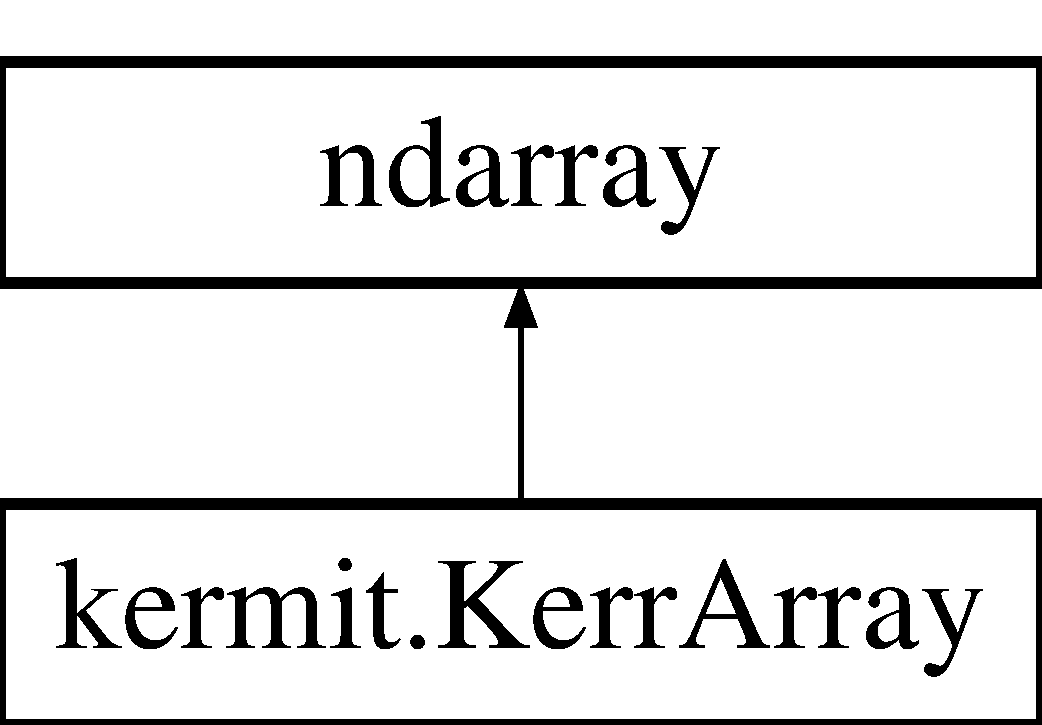
\includegraphics[height=2.000000cm]{classkermit_1_1_kerr_array}
\end{center}
\end{figure}
\subsection*{Public Member Functions}
\begin{DoxyCompactItemize}
\item 
def \hyperlink{classkermit_1_1_kerr_array_a49510d2889f5aef6fa2c67b84396ad64}{\+\_\+\+\_\+new\+\_\+\+\_\+} (cls, image, \hyperlink{classkermit_1_1_kerr_array_a884b10ce1536dc07c4a9ac9346976c22}{metadata}=\{\})
\item 
def \hyperlink{classkermit_1_1_kerr_array_a1d0f724e476ff8264260969898f58a87}{\+\_\+\+\_\+init\+\_\+\+\_\+} (self)
\item 
def \hyperlink{classkermit_1_1_kerr_array_ae0a969a698622942ef4862904736f51b}{\+\_\+\+\_\+array\+\_\+finalize\+\_\+\+\_\+} (self, obj)
\item 
def \hyperlink{classkermit_1_1_kerr_array_adc90cc2f8a25a7366bc0e88a34758186}{\+\_\+\+\_\+array\+\_\+wrap\+\_\+\+\_\+} (self, out\+\_\+arr, context=None)
\item 
def \hyperlink{classkermit_1_1_kerr_array_ac8a4487e7a6dabd4221606d739effe73}{crop\+\_\+text} (self, copy=False)
\item 
def \hyperlink{classkermit_1_1_kerr_array_a0c5f761be9b5daff8773d8c8542c8ba8}{crop\+\_\+image} (self, coord=None, copy=True)
\item 
def \hyperlink{classkermit_1_1_kerr_array_a080a470ae97aa2b99fb2c6a9501da615}{level\+\_\+image} (self, poly\+\_\+vert=1, poly\+\_\+horiz=1, box=None, poly=None)
\item 
def \hyperlink{classkermit_1_1_kerr_array_aecac9b5c400f7397b533262865001665}{get\+\_\+metadata} (self, field\+\_\+only=False)
\item 
def \hyperlink{classkermit_1_1_kerr_array_a7007ac8134bdaccc365e7f88f2c86fa2}{trace} (self, start, end, width=1, order=1)
\item 
def \hyperlink{classkermit_1_1_kerr_array_a09a8c48b921dc96a0134475f6a945b81}{filter\+\_\+image} (self, sigma=2, box=None)
\item 
def \hyperlink{classkermit_1_1_kerr_array_aadeee0dee3e204dacf275d249b44d042}{translate} (self, translation)
\item 
def \hyperlink{classkermit_1_1_kerr_array_a0c8ee5a6ca37169116cd5bc0e70f5f43}{rotate} (self, rotation)
\item 
def \hyperlink{classkermit_1_1_kerr_array_a77d7327a33b40fe6b081b47657cc35fb}{translate\+\_\+limits} (self, translation)
\item 
def \hyperlink{classkermit_1_1_kerr_array_a8b4eaca8f105f02d3d2c4a5af46d3d13}{split\+\_\+image} (self)
\item 
def \hyperlink{classkermit_1_1_kerr_array_adbbf4ec4d3de79f7a8f44b5a4449b07a}{edge\+\_\+det} (filename, threshold1, threshold2)
\item 
def \hyperlink{classkermit_1_1_kerr_array_a5e085bfa80a26a2a16d16c2ba6f86344}{N\+P\+Pixel\+\_\+\+BW} (np\+\_\+image, thresh1, thresh2)
\end{DoxyCompactItemize}
\subsection*{Public Attributes}
\begin{DoxyCompactItemize}
\item 
\hyperlink{classkermit_1_1_kerr_array_a884b10ce1536dc07c4a9ac9346976c22}{metadata}
\item 
\hyperlink{classkermit_1_1_kerr_array_af46ae97efa0085db5e4ed9511ebac823}{shape}
\end{DoxyCompactItemize}


\subsection{Detailed Description}
\begin{DoxyVerb}Class for manipulating Kerr images from Evico software.
It is built to be almost identical to a numpy array except for one extra
parameter which is the metadata. This stores information about the image
in a dictionary object for later retrieval. 
All standard numpy functions should work as normal and casting two types
together should yield a KerrArray type (ie. KerrArray+np.ndarray=KerrArray)

A note on coordinate systems:
For arrays the indexing is (row, column). However the normal way to index
an image would be to do (horizontal, vert), which is the opposite.
In KerrArray the coordinate system is chosen similar to skimage. y points 
down x points right and the origin is in the top left corner of the image.
When indexing the array therefore you need to give it (y,x) coordinates
for (row, column).

 ----> x (column)
|
|
v
y (row)

eg I want the 4th pixel in the horizontal direction and the 10th pixel down
from the top I would ask for KerrArray[10,4]\end{DoxyVerb}
 

\subsection{Constructor \& Destructor Documentation}
\index{kermit\+::\+Kerr\+Array@{kermit\+::\+Kerr\+Array}!\+\_\+\+\_\+init\+\_\+\+\_\+@{\+\_\+\+\_\+init\+\_\+\+\_\+}}
\index{\+\_\+\+\_\+init\+\_\+\+\_\+@{\+\_\+\+\_\+init\+\_\+\+\_\+}!kermit\+::\+Kerr\+Array@{kermit\+::\+Kerr\+Array}}
\subsubsection[{\texorpdfstring{\+\_\+\+\_\+init\+\_\+\+\_\+(self)}{__init__(self)}}]{\setlength{\rightskip}{0pt plus 5cm}def kermit.\+Kerr\+Array.\+\_\+\+\_\+init\+\_\+\+\_\+ (
\begin{DoxyParamCaption}
\item[{}]{self}
\end{DoxyParamCaption}
)}\hypertarget{classkermit_1_1_kerr_array_a1d0f724e476ff8264260969898f58a87}{}\label{classkermit_1_1_kerr_array_a1d0f724e476ff8264260969898f58a87}
\begin{DoxyVerb}called by __new__ when it has finished\end{DoxyVerb}
 

\subsection{Member Function Documentation}
\index{kermit\+::\+Kerr\+Array@{kermit\+::\+Kerr\+Array}!\+\_\+\+\_\+array\+\_\+finalize\+\_\+\+\_\+@{\+\_\+\+\_\+array\+\_\+finalize\+\_\+\+\_\+}}
\index{\+\_\+\+\_\+array\+\_\+finalize\+\_\+\+\_\+@{\+\_\+\+\_\+array\+\_\+finalize\+\_\+\+\_\+}!kermit\+::\+Kerr\+Array@{kermit\+::\+Kerr\+Array}}
\subsubsection[{\texorpdfstring{\+\_\+\+\_\+array\+\_\+finalize\+\_\+\+\_\+(self, obj)}{__array_finalize__(self, obj)}}]{\setlength{\rightskip}{0pt plus 5cm}def kermit.\+Kerr\+Array.\+\_\+\+\_\+array\+\_\+finalize\+\_\+\+\_\+ (
\begin{DoxyParamCaption}
\item[{}]{self, }
\item[{}]{obj}
\end{DoxyParamCaption}
)}\hypertarget{classkermit_1_1_kerr_array_ae0a969a698622942ef4862904736f51b}{}\label{classkermit_1_1_kerr_array_ae0a969a698622942ef4862904736f51b}
\begin{DoxyVerb}__array_finalize__ and __array_wrap__ are necessary functions when
subclassing numpy.ndarray to fix some behaviours. See
http://docs.scipy.org/doc/numpy-1.10.1/user/basics.subclassing.html for
more info and examples
\end{DoxyVerb}
 \index{kermit\+::\+Kerr\+Array@{kermit\+::\+Kerr\+Array}!\+\_\+\+\_\+array\+\_\+wrap\+\_\+\+\_\+@{\+\_\+\+\_\+array\+\_\+wrap\+\_\+\+\_\+}}
\index{\+\_\+\+\_\+array\+\_\+wrap\+\_\+\+\_\+@{\+\_\+\+\_\+array\+\_\+wrap\+\_\+\+\_\+}!kermit\+::\+Kerr\+Array@{kermit\+::\+Kerr\+Array}}
\subsubsection[{\texorpdfstring{\+\_\+\+\_\+array\+\_\+wrap\+\_\+\+\_\+(self, out\+\_\+arr, context=\+None)}{__array_wrap__(self, out_arr, context=None)}}]{\setlength{\rightskip}{0pt plus 5cm}def kermit.\+Kerr\+Array.\+\_\+\+\_\+array\+\_\+wrap\+\_\+\+\_\+ (
\begin{DoxyParamCaption}
\item[{}]{self, }
\item[{}]{out\+\_\+arr, }
\item[{}]{context = {\ttfamily None}}
\end{DoxyParamCaption}
)}\hypertarget{classkermit_1_1_kerr_array_adc90cc2f8a25a7366bc0e88a34758186}{}\label{classkermit_1_1_kerr_array_adc90cc2f8a25a7366bc0e88a34758186}
\begin{DoxyVerb}see __array_finalize__ for info\end{DoxyVerb}
 \index{kermit\+::\+Kerr\+Array@{kermit\+::\+Kerr\+Array}!\+\_\+\+\_\+new\+\_\+\+\_\+@{\+\_\+\+\_\+new\+\_\+\+\_\+}}
\index{\+\_\+\+\_\+new\+\_\+\+\_\+@{\+\_\+\+\_\+new\+\_\+\+\_\+}!kermit\+::\+Kerr\+Array@{kermit\+::\+Kerr\+Array}}
\subsubsection[{\texorpdfstring{\+\_\+\+\_\+new\+\_\+\+\_\+(cls, image, metadata=\lcurly{}\rcurly{})}{__new__(cls, image, metadata=\{\})}}]{\setlength{\rightskip}{0pt plus 5cm}def kermit.\+Kerr\+Array.\+\_\+\+\_\+new\+\_\+\+\_\+ (
\begin{DoxyParamCaption}
\item[{}]{cls, }
\item[{}]{image, }
\item[{}]{metadata = {\ttfamily \{\}}}
\end{DoxyParamCaption}
)}\hypertarget{classkermit_1_1_kerr_array_a49510d2889f5aef6fa2c67b84396ad64}{}\label{classkermit_1_1_kerr_array_a49510d2889f5aef6fa2c67b84396ad64}
\begin{DoxyVerb}Construct a Kermit object. We're using __new__ rather than __init__
to imitate a numpy array as close as possible.

Parameters
----------
image: string or numpy array initiator
    If a filename is given it will try to load the image from memory
    Otherwise it will call np.array(image) on the object so an array or
    list is suitable
metadata: dict
    dictionary of metadata items you would like adding to your array
Returns
-------
ka: KerrArray
    A KerrArray object with metadata attached
\end{DoxyVerb}
 \index{kermit\+::\+Kerr\+Array@{kermit\+::\+Kerr\+Array}!crop\+\_\+image@{crop\+\_\+image}}
\index{crop\+\_\+image@{crop\+\_\+image}!kermit\+::\+Kerr\+Array@{kermit\+::\+Kerr\+Array}}
\subsubsection[{\texorpdfstring{crop\+\_\+image(self, coord=\+None, copy=\+True)}{crop_image(self, coord=None, copy=True)}}]{\setlength{\rightskip}{0pt plus 5cm}def kermit.\+Kerr\+Array.\+crop\+\_\+image (
\begin{DoxyParamCaption}
\item[{}]{self, }
\item[{}]{coord = {\ttfamily None}, }
\item[{}]{copy = {\ttfamily True}}
\end{DoxyParamCaption}
)}\hypertarget{classkermit_1_1_kerr_array_a0c5f761be9b5daff8773d8c8542c8ba8}{}\label{classkermit_1_1_kerr_array_a0c5f761be9b5daff8773d8c8542c8ba8}
\begin{DoxyVerb}Crop the image. 
Crops to the coord given or defaults to allowing the user
to draw a rectangle. Returns the cropped image.

Parameters
----------
coord: array or list of type int:  
    [xmin,xmax,ymin,ymax]
copy: bool
    whether to return a copy of the array or a view of the original object

Returns
-------
im: KerrArray
    cropped image
\end{DoxyVerb}
 \index{kermit\+::\+Kerr\+Array@{kermit\+::\+Kerr\+Array}!crop\+\_\+text@{crop\+\_\+text}}
\index{crop\+\_\+text@{crop\+\_\+text}!kermit\+::\+Kerr\+Array@{kermit\+::\+Kerr\+Array}}
\subsubsection[{\texorpdfstring{crop\+\_\+text(self, copy=\+False)}{crop_text(self, copy=False)}}]{\setlength{\rightskip}{0pt plus 5cm}def kermit.\+Kerr\+Array.\+crop\+\_\+text (
\begin{DoxyParamCaption}
\item[{}]{self, }
\item[{}]{copy = {\ttfamily False}}
\end{DoxyParamCaption}
)}\hypertarget{classkermit_1_1_kerr_array_ac8a4487e7a6dabd4221606d739effe73}{}\label{classkermit_1_1_kerr_array_ac8a4487e7a6dabd4221606d739effe73}
\begin{DoxyVerb}Crop the bottom text area from a standard Kermit image

Parameters
----------
copy: bool
    Whether to return a copy of the data or the original data

Returns
-------
im: KerrArray
    cropped image           
\end{DoxyVerb}
 \index{kermit\+::\+Kerr\+Array@{kermit\+::\+Kerr\+Array}!edge\+\_\+det@{edge\+\_\+det}}
\index{edge\+\_\+det@{edge\+\_\+det}!kermit\+::\+Kerr\+Array@{kermit\+::\+Kerr\+Array}}
\subsubsection[{\texorpdfstring{edge\+\_\+det(filename, threshold1, threshold2)}{edge_det(filename, threshold1, threshold2)}}]{\setlength{\rightskip}{0pt plus 5cm}def kermit.\+Kerr\+Array.\+edge\+\_\+det (
\begin{DoxyParamCaption}
\item[{}]{filename, }
\item[{}]{threshold1, }
\item[{}]{threshold2}
\end{DoxyParamCaption}
)}\hypertarget{classkermit_1_1_kerr_array_adbbf4ec4d3de79f7a8f44b5a4449b07a}{}\label{classkermit_1_1_kerr_array_adbbf4ec4d3de79f7a8f44b5a4449b07a}
\begin{DoxyVerb}Detects an edges in an image according to the thresholds 1 and 2.
Below threshold 1, a pixel is disregarded from the edge
Above threshold 2, pixels contribute to the edge
Inbetween 1&2, if the pixel is connected to similar pixels then the pixel conributes to the edge \end{DoxyVerb}
 \index{kermit\+::\+Kerr\+Array@{kermit\+::\+Kerr\+Array}!filter\+\_\+image@{filter\+\_\+image}}
\index{filter\+\_\+image@{filter\+\_\+image}!kermit\+::\+Kerr\+Array@{kermit\+::\+Kerr\+Array}}
\subsubsection[{\texorpdfstring{filter\+\_\+image(self, sigma=2, box=\+None)}{filter_image(self, sigma=2, box=None)}}]{\setlength{\rightskip}{0pt plus 5cm}def kermit.\+Kerr\+Array.\+filter\+\_\+image (
\begin{DoxyParamCaption}
\item[{}]{self, }
\item[{}]{sigma = {\ttfamily 2}, }
\item[{}]{box = {\ttfamily None}}
\end{DoxyParamCaption}
)}\hypertarget{classkermit_1_1_kerr_array_a09a8c48b921dc96a0134475f6a945b81}{}\label{classkermit_1_1_kerr_array_a09a8c48b921dc96a0134475f6a945b81}
\begin{DoxyVerb}Apply a filter to an area of the image defined by box
call through to skimage.filters.gaussian

Parameters
----------
sigma: float
    standard deviation for gaussian blur
box: 4-tuple
    area to apply blur to (xmin,xmax,ymin,ymax)

Returns
-------
image
    filtered image
\end{DoxyVerb}
 \index{kermit\+::\+Kerr\+Array@{kermit\+::\+Kerr\+Array}!get\+\_\+metadata@{get\+\_\+metadata}}
\index{get\+\_\+metadata@{get\+\_\+metadata}!kermit\+::\+Kerr\+Array@{kermit\+::\+Kerr\+Array}}
\subsubsection[{\texorpdfstring{get\+\_\+metadata(self, field\+\_\+only=\+False)}{get_metadata(self, field_only=False)}}]{\setlength{\rightskip}{0pt plus 5cm}def kermit.\+Kerr\+Array.\+get\+\_\+metadata (
\begin{DoxyParamCaption}
\item[{}]{self, }
\item[{}]{field\+\_\+only = {\ttfamily False}}
\end{DoxyParamCaption}
)}\hypertarget{classkermit_1_1_kerr_array_aecac9b5c400f7397b533262865001665}{}\label{classkermit_1_1_kerr_array_aecac9b5c400f7397b533262865001665}
\begin{DoxyVerb}Use image recognition to try to pull the metadata numbers off the image

Requirements: This function uses tesseract to recognise the image, therefore
tesseract file1 file2 must be valid on your command line.
Install tesseract from 
https://sourceforge.net/projects/tesseract-ocr-alt/files/?source=navbar
    
Parameters
----------
field_only: bool
    only try to return a field value

Returns
-------
metadata: dict
    updated metadata dictionary
\end{DoxyVerb}
 \index{kermit\+::\+Kerr\+Array@{kermit\+::\+Kerr\+Array}!level\+\_\+image@{level\+\_\+image}}
\index{level\+\_\+image@{level\+\_\+image}!kermit\+::\+Kerr\+Array@{kermit\+::\+Kerr\+Array}}
\subsubsection[{\texorpdfstring{level\+\_\+image(self, poly\+\_\+vert=1, poly\+\_\+horiz=1, box=\+None, poly=\+None)}{level_image(self, poly_vert=1, poly_horiz=1, box=None, poly=None)}}]{\setlength{\rightskip}{0pt plus 5cm}def kermit.\+Kerr\+Array.\+level\+\_\+image (
\begin{DoxyParamCaption}
\item[{}]{self, }
\item[{}]{poly\+\_\+vert = {\ttfamily 1}, }
\item[{}]{poly\+\_\+horiz = {\ttfamily 1}, }
\item[{}]{box = {\ttfamily None}, }
\item[{}]{poly = {\ttfamily None}}
\end{DoxyParamCaption}
)}\hypertarget{classkermit_1_1_kerr_array_a080a470ae97aa2b99fb2c6a9501da615}{}\label{classkermit_1_1_kerr_array_a080a470ae97aa2b99fb2c6a9501da615}
\begin{DoxyVerb}Subtract a polynomial background from image

Fit and subtract a background to the image. Fits a polynomial of order
given in the horizontal and vertical directions and subtracts. If box 
is defined then level the *entire* image according to the 
gradient within the box.

Parameters
----------
poly_vert: int
    fit a polynomial in the vertical direction for the image of order 
    given. If 0 do not fit or subtract in the vertical direction
poly_horiz: int
    fit a polynomial of order poly_horiz to the image. If 0 given
    do not subtract
box: array, list or tuple of int
    [xmin,xmax,ymin,ymax] define region for fitting. IF None use entire
    image
poly: list or None
    [pvert, phoriz] pvert and phoriz are arrays of polynomial coefficients
    (highest power first) to subtract in the horizontal and vertical 
    directions. If None function defaults to fitting its own polynomial.
    
Returns
-------
im: KerrArray
    the levelled image
\end{DoxyVerb}
 \index{kermit\+::\+Kerr\+Array@{kermit\+::\+Kerr\+Array}!N\+P\+Pixel\+\_\+\+BW@{N\+P\+Pixel\+\_\+\+BW}}
\index{N\+P\+Pixel\+\_\+\+BW@{N\+P\+Pixel\+\_\+\+BW}!kermit\+::\+Kerr\+Array@{kermit\+::\+Kerr\+Array}}
\subsubsection[{\texorpdfstring{N\+P\+Pixel\+\_\+\+B\+W(np\+\_\+image, thresh1, thresh2)}{NPPixel_BW(np_image, thresh1, thresh2)}}]{\setlength{\rightskip}{0pt plus 5cm}def kermit.\+Kerr\+Array.\+N\+P\+Pixel\+\_\+\+BW (
\begin{DoxyParamCaption}
\item[{}]{np\+\_\+image, }
\item[{}]{thresh1, }
\item[{}]{thresh2}
\end{DoxyParamCaption}
)}\hypertarget{classkermit_1_1_kerr_array_a5e085bfa80a26a2a16d16c2ba6f86344}{}\label{classkermit_1_1_kerr_array_a5e085bfa80a26a2a16d16c2ba6f86344}
\begin{DoxyVerb}Changes the colour if pixels in a np array according to an inputted threshold\end{DoxyVerb}
 \index{kermit\+::\+Kerr\+Array@{kermit\+::\+Kerr\+Array}!rotate@{rotate}}
\index{rotate@{rotate}!kermit\+::\+Kerr\+Array@{kermit\+::\+Kerr\+Array}}
\subsubsection[{\texorpdfstring{rotate(self, rotation)}{rotate(self, rotation)}}]{\setlength{\rightskip}{0pt plus 5cm}def kermit.\+Kerr\+Array.\+rotate (
\begin{DoxyParamCaption}
\item[{}]{self, }
\item[{}]{rotation}
\end{DoxyParamCaption}
)}\hypertarget{classkermit_1_1_kerr_array_a0c8ee5a6ca37169116cd5bc0e70f5f43}{}\label{classkermit_1_1_kerr_array_a0c8ee5a6ca37169116cd5bc0e70f5f43}
\begin{DoxyVerb}Rotates the image.
Areas lost by move are cropped, and areas gained are made black (0)

Parameters
----------
rotation: float
    clockwise rotation angle in radians (rotated about top right corner)

Returns
-------
im: KerrArray
    rotated image
\end{DoxyVerb}
 \index{kermit\+::\+Kerr\+Array@{kermit\+::\+Kerr\+Array}!split\+\_\+image@{split\+\_\+image}}
\index{split\+\_\+image@{split\+\_\+image}!kermit\+::\+Kerr\+Array@{kermit\+::\+Kerr\+Array}}
\subsubsection[{\texorpdfstring{split\+\_\+image(self)}{split_image(self)}}]{\setlength{\rightskip}{0pt plus 5cm}def kermit.\+Kerr\+Array.\+split\+\_\+image (
\begin{DoxyParamCaption}
\item[{}]{self}
\end{DoxyParamCaption}
)}\hypertarget{classkermit_1_1_kerr_array_a8b4eaca8f105f02d3d2c4a5af46d3d13}{}\label{classkermit_1_1_kerr_array_a8b4eaca8f105f02d3d2c4a5af46d3d13}
\begin{DoxyVerb}split image into different domains, maybe by peak fitting the histogram?\end{DoxyVerb}
 \index{kermit\+::\+Kerr\+Array@{kermit\+::\+Kerr\+Array}!trace@{trace}}
\index{trace@{trace}!kermit\+::\+Kerr\+Array@{kermit\+::\+Kerr\+Array}}
\subsubsection[{\texorpdfstring{trace(self, start, end, width=1, order=1)}{trace(self, start, end, width=1, order=1)}}]{\setlength{\rightskip}{0pt plus 5cm}def kermit.\+Kerr\+Array.\+trace (
\begin{DoxyParamCaption}
\item[{}]{self, }
\item[{}]{start, }
\item[{}]{end, }
\item[{}]{width = {\ttfamily 1}, }
\item[{}]{order = {\ttfamily 1}}
\end{DoxyParamCaption}
)}\hypertarget{classkermit_1_1_kerr_array_a7007ac8134bdaccc365e7f88f2c86fa2}{}\label{classkermit_1_1_kerr_array_a7007ac8134bdaccc365e7f88f2c86fa2}
\begin{DoxyVerb}Return a line trace of intensity averaging over width.
Call through to skimage.measure.profile_line

Parameters
----------
start: 2-tuple
    coords at start of line (numpy coordinates not x,y)
end: 2-tuple
    coords at end of line (last pixel is included in result)
width: int
    width of line to average over
order: int
    order of the spline interpolation

Returns
-------
profile: array
    intensity profile
\end{DoxyVerb}
 \index{kermit\+::\+Kerr\+Array@{kermit\+::\+Kerr\+Array}!translate@{translate}}
\index{translate@{translate}!kermit\+::\+Kerr\+Array@{kermit\+::\+Kerr\+Array}}
\subsubsection[{\texorpdfstring{translate(self, translation)}{translate(self, translation)}}]{\setlength{\rightskip}{0pt plus 5cm}def kermit.\+Kerr\+Array.\+translate (
\begin{DoxyParamCaption}
\item[{}]{self, }
\item[{}]{translation}
\end{DoxyParamCaption}
)}\hypertarget{classkermit_1_1_kerr_array_aadeee0dee3e204dacf275d249b44d042}{}\label{classkermit_1_1_kerr_array_aadeee0dee3e204dacf275d249b44d042}
\begin{DoxyVerb}Translates the image.
Areas lost by move are cropped, and areas gained are made black (0)

Parameters
----------
translate: 2-tuple
    translation (x,y)

Returns
-------
im: KerrArray
    translated image
\end{DoxyVerb}
 \index{kermit\+::\+Kerr\+Array@{kermit\+::\+Kerr\+Array}!translate\+\_\+limits@{translate\+\_\+limits}}
\index{translate\+\_\+limits@{translate\+\_\+limits}!kermit\+::\+Kerr\+Array@{kermit\+::\+Kerr\+Array}}
\subsubsection[{\texorpdfstring{translate\+\_\+limits(self, translation)}{translate_limits(self, translation)}}]{\setlength{\rightskip}{0pt plus 5cm}def kermit.\+Kerr\+Array.\+translate\+\_\+limits (
\begin{DoxyParamCaption}
\item[{}]{self, }
\item[{}]{translation}
\end{DoxyParamCaption}
)}\hypertarget{classkermit_1_1_kerr_array_a77d7327a33b40fe6b081b47657cc35fb}{}\label{classkermit_1_1_kerr_array_a77d7327a33b40fe6b081b47657cc35fb}
\begin{DoxyVerb}Find the limits of an image after a translation
After using KerrArray.translate some areas will be black,
this finds the area that still has original pixels in

Parameters
----------
translation: 2 tuple
    the (x,y) translation applied to the image

Returns
-------
limits: 4-tuple
    (xmin,xmax,ymin,ymax\end{DoxyVerb}
 

\subsection{Member Data Documentation}
\index{kermit\+::\+Kerr\+Array@{kermit\+::\+Kerr\+Array}!metadata@{metadata}}
\index{metadata@{metadata}!kermit\+::\+Kerr\+Array@{kermit\+::\+Kerr\+Array}}
\subsubsection[{\texorpdfstring{metadata}{metadata}}]{\setlength{\rightskip}{0pt plus 5cm}kermit.\+Kerr\+Array.\+metadata}\hypertarget{classkermit_1_1_kerr_array_a884b10ce1536dc07c4a9ac9346976c22}{}\label{classkermit_1_1_kerr_array_a884b10ce1536dc07c4a9ac9346976c22}
\index{kermit\+::\+Kerr\+Array@{kermit\+::\+Kerr\+Array}!shape@{shape}}
\index{shape@{shape}!kermit\+::\+Kerr\+Array@{kermit\+::\+Kerr\+Array}}
\subsubsection[{\texorpdfstring{shape}{shape}}]{\setlength{\rightskip}{0pt plus 5cm}kermit.\+Kerr\+Array.\+shape}\hypertarget{classkermit_1_1_kerr_array_af46ae97efa0085db5e4ed9511ebac823}{}\label{classkermit_1_1_kerr_array_af46ae97efa0085db5e4ed9511ebac823}


The documentation for this class was generated from the following file\+:\begin{DoxyCompactItemize}
\item 
C\+:/\+Users/phyrct/\+Dropbox/\+Me/\+Coding/kermit/kermit/\hyperlink{kermit_8py}{kermit.\+py}\end{DoxyCompactItemize}

\hypertarget{classkermit_1_1_kerr_g_u_i}{}\section{kermit.\+Kerr\+G\+UI Class Reference}
\label{classkermit_1_1_kerr_g_u_i}\index{kermit.\+Kerr\+G\+UI@{kermit.\+Kerr\+G\+UI}}
\subsection*{Public Member Functions}
\begin{DoxyCompactItemize}
\item 
def \hyperlink{classkermit_1_1_kerr_g_u_i_a081d6dc01ab9df34b2b74622d8a93bd9}{draw\+\_\+rectangle} (self)
\item 
def \hyperlink{classkermit_1_1_kerr_g_u_i_a28fde831d88f3bd1b44adaf745ccee83}{draw\+\_\+trace} (vert\+\_\+coord, width=1)
\item 
def \hyperlink{classkermit_1_1_kerr_g_u_i_aad0003940aa88ea501243f1e65c30485}{plt\+\_\+histogram} (self, kwarg)
\end{DoxyCompactItemize}


\subsection{Member Function Documentation}
\index{kermit\+::\+Kerr\+G\+UI@{kermit\+::\+Kerr\+G\+UI}!draw\+\_\+rectangle@{draw\+\_\+rectangle}}
\index{draw\+\_\+rectangle@{draw\+\_\+rectangle}!kermit\+::\+Kerr\+G\+UI@{kermit\+::\+Kerr\+G\+UI}}
\subsubsection[{\texorpdfstring{draw\+\_\+rectangle(self)}{draw_rectangle(self)}}]{\setlength{\rightskip}{0pt plus 5cm}def kermit.\+Kerr\+G\+U\+I.\+draw\+\_\+rectangle (
\begin{DoxyParamCaption}
\item[{}]{self}
\end{DoxyParamCaption}
)}\hypertarget{classkermit_1_1_kerr_g_u_i_a081d6dc01ab9df34b2b74622d8a93bd9}{}\label{classkermit_1_1_kerr_g_u_i_a081d6dc01ab9df34b2b74622d8a93bd9}
\begin{DoxyVerb}Draw a rectangle on the image and return the coordinates

Returns
-------
coord: ndarray
    [xmin,xmax,ymin,ymax]\end{DoxyVerb}
 \index{kermit\+::\+Kerr\+G\+UI@{kermit\+::\+Kerr\+G\+UI}!draw\+\_\+trace@{draw\+\_\+trace}}
\index{draw\+\_\+trace@{draw\+\_\+trace}!kermit\+::\+Kerr\+G\+UI@{kermit\+::\+Kerr\+G\+UI}}
\subsubsection[{\texorpdfstring{draw\+\_\+trace(vert\+\_\+coord, width=1)}{draw_trace(vert_coord, width=1)}}]{\setlength{\rightskip}{0pt plus 5cm}def kermit.\+Kerr\+G\+U\+I.\+draw\+\_\+trace (
\begin{DoxyParamCaption}
\item[{}]{vert\+\_\+coord, }
\item[{}]{width = {\ttfamily 1}}
\end{DoxyParamCaption}
)}\hypertarget{classkermit_1_1_kerr_g_u_i_a28fde831d88f3bd1b44adaf745ccee83}{}\label{classkermit_1_1_kerr_g_u_i_a28fde831d88f3bd1b44adaf745ccee83}
\begin{DoxyVerb}Line trace horizontal at vertical coord averaging over width\end{DoxyVerb}
 \index{kermit\+::\+Kerr\+G\+UI@{kermit\+::\+Kerr\+G\+UI}!plt\+\_\+histogram@{plt\+\_\+histogram}}
\index{plt\+\_\+histogram@{plt\+\_\+histogram}!kermit\+::\+Kerr\+G\+UI@{kermit\+::\+Kerr\+G\+UI}}
\subsubsection[{\texorpdfstring{plt\+\_\+histogram(self, kwarg)}{plt_histogram(self, kwarg)}}]{\setlength{\rightskip}{0pt plus 5cm}def kermit.\+Kerr\+G\+U\+I.\+plt\+\_\+histogram (
\begin{DoxyParamCaption}
\item[{}]{self, }
\item[{}]{kwarg}
\end{DoxyParamCaption}
)}\hypertarget{classkermit_1_1_kerr_g_u_i_aad0003940aa88ea501243f1e65c30485}{}\label{classkermit_1_1_kerr_g_u_i_aad0003940aa88ea501243f1e65c30485}
\begin{DoxyVerb}plot histogram of image intensities, pass through kwarg to matplotlib.pyplot.hist\end{DoxyVerb}
 

The documentation for this class was generated from the following file\+:\begin{DoxyCompactItemize}
\item 
C\+:/\+Users/phyrct/\+Dropbox/\+Me/\+Coding/kermit/kermit/\hyperlink{kermit_8py}{kermit.\+py}\end{DoxyCompactItemize}

\hypertarget{classkerrlist_1_1_kerr_list}{}\section{kerrlist.\+Kerr\+List Class Reference}
\label{classkerrlist_1_1_kerr_list}\index{kerrlist.\+Kerr\+List@{kerrlist.\+Kerr\+List}}
Inheritance diagram for kerrlist.\+Kerr\+List\+:\begin{figure}[H]
\begin{center}
\leavevmode
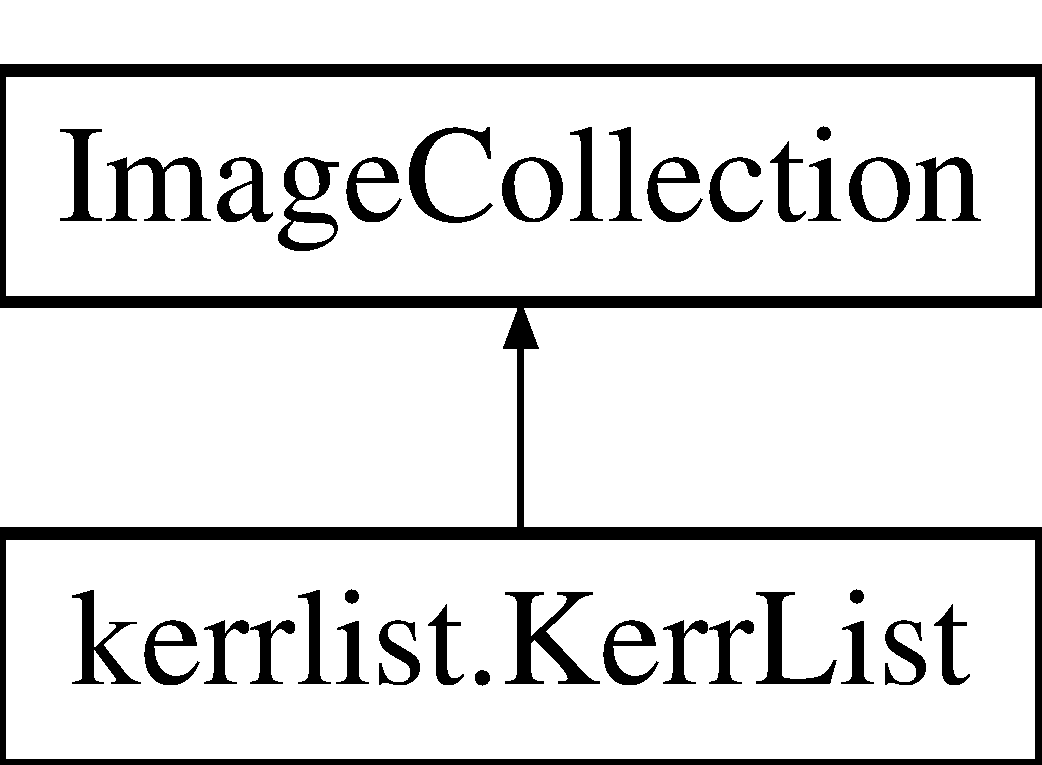
\includegraphics[height=2.000000cm]{classkerrlist_1_1_kerr_list}
\end{center}
\end{figure}
\subsection*{Public Member Functions}
\begin{DoxyCompactItemize}
\item 
def \hyperlink{classkerrlist_1_1_kerr_list_a6f3bf73e2595c3a2a4b2aa49147d405f}{\+\_\+\+\_\+init\+\_\+\+\_\+} (self, load\+\_\+pattern, conserve\+\_\+memory=True, load\+\_\+func=None, load\+\_\+func\+\_\+kwargs)
\item 
def \hyperlink{classkerrlist_1_1_kerr_list_a1a59547bb6113d06a09c615ec065ed44}{hysteresis\+\_\+loop} (self, fieldlist=None, box=None)
\item 
def \hyperlink{classkerrlist_1_1_kerr_list_a278b5b346bae5e1e5780c7805ab9ebac}{drift\+\_\+loop\+\_\+correct} (hysloop, manual=False)
\item 
def \hyperlink{classkerrlist_1_1_kerr_list_aca95a7b5d663e5724fdf2e249c3f1445}{faraday\+\_\+correct} (hysloop, manual=False)
\item 
def \hyperlink{classkerrlist_1_1_kerr_list_a3f84d6f283bf77c30e753fe7c90678f6}{correct\+\_\+image\+\_\+drift} (self, ref, imlist, threshold=0.\+005)
\item 
def \hyperlink{classkerrlist_1_1_kerr_list_a9abcf1aa70e0ac1d003040ff9739acfb}{transform\+\_\+images} (imlist, translation=None, rotation=None)
\end{DoxyCompactItemize}


\subsection{Detailed Description}
\begin{DoxyVerb}KerrList groups functions that can be applied to a group of KerrImages.
In general it is designed to behave pretty much like a normal python list.
\end{DoxyVerb}
 

\subsection{Constructor \& Destructor Documentation}
\index{kerrlist\+::\+Kerr\+List@{kerrlist\+::\+Kerr\+List}!\+\_\+\+\_\+init\+\_\+\+\_\+@{\+\_\+\+\_\+init\+\_\+\+\_\+}}
\index{\+\_\+\+\_\+init\+\_\+\+\_\+@{\+\_\+\+\_\+init\+\_\+\+\_\+}!kerrlist\+::\+Kerr\+List@{kerrlist\+::\+Kerr\+List}}
\subsubsection[{\texorpdfstring{\+\_\+\+\_\+init\+\_\+\+\_\+(self, load\+\_\+pattern, conserve\+\_\+memory=\+True, load\+\_\+func=\+None, load\+\_\+func\+\_\+kwargs)}{__init__(self, load_pattern, conserve_memory=True, load_func=None, load_func_kwargs)}}]{\setlength{\rightskip}{0pt plus 5cm}def kerrlist.\+Kerr\+List.\+\_\+\+\_\+init\+\_\+\+\_\+ (
\begin{DoxyParamCaption}
\item[{}]{self, }
\item[{}]{load\+\_\+pattern, }
\item[{}]{conserve\+\_\+memory = {\ttfamily True}, }
\item[{}]{load\+\_\+func = {\ttfamily None}, }
\item[{}]{load\+\_\+func\+\_\+kwargs}
\end{DoxyParamCaption}
)}\hypertarget{classkerrlist_1_1_kerr_list_a6f3bf73e2595c3a2a4b2aa49147d405f}{}\label{classkerrlist_1_1_kerr_list_a6f3bf73e2595c3a2a4b2aa49147d405f}
\begin{DoxyVerb}Initialise a KerrList. A list of images to manipulate. Mostly a pass
through to the skimage.io.ImageCollection class

Parameters
----------
load_pattern: str or list
    pattern of filenames to load. Uses standard glob nomenclature. Seperate
    different requests with a : eg 'myimages/*.png:myimages/*.jpg'. If
    a list is given it treats it as a list of image arrays.
pattern: str or list
    loading pattern with standard glob nomenclature (* wildcards, 
    [0-9] character in this range etc.)
conserve_memory: bool
    parameter passed onto skimage.io.ImageCollection. Option for loading
    all the files into memory initially or later

Other parameters
----------------
load_func: callable or None
    see skimage.io.ImageCollection for notes.

Attributes
----------
files: list or str
    list of loaded file names. Or equal to load_pattern if a list was
    given.\end{DoxyVerb}
 

\subsection{Member Function Documentation}
\index{kerrlist\+::\+Kerr\+List@{kerrlist\+::\+Kerr\+List}!correct\+\_\+image\+\_\+drift@{correct\+\_\+image\+\_\+drift}}
\index{correct\+\_\+image\+\_\+drift@{correct\+\_\+image\+\_\+drift}!kerrlist\+::\+Kerr\+List@{kerrlist\+::\+Kerr\+List}}
\subsubsection[{\texorpdfstring{correct\+\_\+image\+\_\+drift(self, ref, imlist, threshold=0.\+005)}{correct_image_drift(self, ref, imlist, threshold=0.005)}}]{\setlength{\rightskip}{0pt plus 5cm}def kerrlist.\+Kerr\+List.\+correct\+\_\+image\+\_\+drift (
\begin{DoxyParamCaption}
\item[{}]{self, }
\item[{}]{ref, }
\item[{}]{imlist, }
\item[{}]{threshold = {\ttfamily 0.005}}
\end{DoxyParamCaption}
)}\hypertarget{classkerrlist_1_1_kerr_list_a3f84d6f283bf77c30e753fe7c90678f6}{}\label{classkerrlist_1_1_kerr_list_a3f84d6f283bf77c30e753fe7c90678f6}
\begin{DoxyVerb}Align images to correct for image drift.
Detects common features on the images and tracks them moving.

Parameters
----------
ref: np.ndarry
    reference image with zero drift
imlist: list or tuple of images
    images to find drift
threshold: float
    threshold for detecting imperfections in images

Returns
-------
shifts: array
    shift vector for each image in imlist relative to ref (x drift, y drift)
transim: list
    list of images with correct shifts applied\end{DoxyVerb}
 \index{kerrlist\+::\+Kerr\+List@{kerrlist\+::\+Kerr\+List}!drift\+\_\+loop\+\_\+correct@{drift\+\_\+loop\+\_\+correct}}
\index{drift\+\_\+loop\+\_\+correct@{drift\+\_\+loop\+\_\+correct}!kerrlist\+::\+Kerr\+List@{kerrlist\+::\+Kerr\+List}}
\subsubsection[{\texorpdfstring{drift\+\_\+loop\+\_\+correct(hysloop, manual=\+False)}{drift_loop_correct(hysloop, manual=False)}}]{\setlength{\rightskip}{0pt plus 5cm}def kerrlist.\+Kerr\+List.\+drift\+\_\+loop\+\_\+correct (
\begin{DoxyParamCaption}
\item[{}]{hysloop, }
\item[{}]{manual = {\ttfamily False}}
\end{DoxyParamCaption}
)}\hypertarget{classkerrlist_1_1_kerr_list_a278b5b346bae5e1e5780c7805ab9ebac}{}\label{classkerrlist_1_1_kerr_list_a278b5b346bae5e1e5780c7805ab9ebac}
\begin{DoxyVerb}correct a linear drift in time on a hysteresis loop\end{DoxyVerb}
 \index{kerrlist\+::\+Kerr\+List@{kerrlist\+::\+Kerr\+List}!faraday\+\_\+correct@{faraday\+\_\+correct}}
\index{faraday\+\_\+correct@{faraday\+\_\+correct}!kerrlist\+::\+Kerr\+List@{kerrlist\+::\+Kerr\+List}}
\subsubsection[{\texorpdfstring{faraday\+\_\+correct(hysloop, manual=\+False)}{faraday_correct(hysloop, manual=False)}}]{\setlength{\rightskip}{0pt plus 5cm}def kerrlist.\+Kerr\+List.\+faraday\+\_\+correct (
\begin{DoxyParamCaption}
\item[{}]{hysloop, }
\item[{}]{manual = {\ttfamily False}}
\end{DoxyParamCaption}
)}\hypertarget{classkerrlist_1_1_kerr_list_aca95a7b5d663e5724fdf2e249c3f1445}{}\label{classkerrlist_1_1_kerr_list_aca95a7b5d663e5724fdf2e249c3f1445}
\begin{DoxyVerb}correct for the faraday effect\end{DoxyVerb}
 \index{kerrlist\+::\+Kerr\+List@{kerrlist\+::\+Kerr\+List}!hysteresis\+\_\+loop@{hysteresis\+\_\+loop}}
\index{hysteresis\+\_\+loop@{hysteresis\+\_\+loop}!kerrlist\+::\+Kerr\+List@{kerrlist\+::\+Kerr\+List}}
\subsubsection[{\texorpdfstring{hysteresis\+\_\+loop(self, fieldlist=\+None, box=\+None)}{hysteresis_loop(self, fieldlist=None, box=None)}}]{\setlength{\rightskip}{0pt plus 5cm}def kerrlist.\+Kerr\+List.\+hysteresis\+\_\+loop (
\begin{DoxyParamCaption}
\item[{}]{self, }
\item[{}]{fieldlist = {\ttfamily None}, }
\item[{}]{box = {\ttfamily None}}
\end{DoxyParamCaption}
)}\hypertarget{classkerrlist_1_1_kerr_list_a1a59547bb6113d06a09c615ec065ed44}{}\label{classkerrlist_1_1_kerr_list_a1a59547bb6113d06a09c615ec065ed44}
\begin{DoxyVerb}Make a hysteresis loop of the average intensity in the given images

Parameters
----------
fieldlist: list or tuple 
    list of fields used, if None it will try to get field from imgae metadata
box: list 
    [xmin,xmax,ymin,ymax] region of interest for hysteresis\end{DoxyVerb}
 \index{kerrlist\+::\+Kerr\+List@{kerrlist\+::\+Kerr\+List}!transform\+\_\+images@{transform\+\_\+images}}
\index{transform\+\_\+images@{transform\+\_\+images}!kerrlist\+::\+Kerr\+List@{kerrlist\+::\+Kerr\+List}}
\subsubsection[{\texorpdfstring{transform\+\_\+images(imlist, translation=\+None, rotation=\+None)}{transform_images(imlist, translation=None, rotation=None)}}]{\setlength{\rightskip}{0pt plus 5cm}def kerrlist.\+Kerr\+List.\+transform\+\_\+images (
\begin{DoxyParamCaption}
\item[{}]{imlist, }
\item[{}]{translation = {\ttfamily None}, }
\item[{}]{rotation = {\ttfamily None}}
\end{DoxyParamCaption}
)}\hypertarget{classkerrlist_1_1_kerr_list_a9abcf1aa70e0ac1d003040ff9739acfb}{}\label{classkerrlist_1_1_kerr_list_a9abcf1aa70e0ac1d003040ff9739acfb}
\begin{DoxyVerb}Translate or rotate image or images. 
Translates or rotates the images in the x-y plane. Areas lost by move are cropped, and 
areas gained are made black.

Parameters
----------
im: array or list
    image or list of images to be translated
tranlations: tuple or list
    array of relative distances for translation [horizontal, vert]
    eg. [[1,3],[-5,4],[9,-8]]. Defaults to no translation
rotations: float or list
    list of rotation angles in radians to apply to the images (rotates about top left
    corner). Defaults to 0.

Returns 
newims: list 
    The transformed images (all of the same shape as the originals)
lims: array
    The limits of the image that have not been destroyed by translations
    [xmin,xmax,ymin,ymax] (doesn't account for rotation yet!)       
\end{DoxyVerb}
 

The documentation for this class was generated from the following file\+:\begin{DoxyCompactItemize}
\item 
C\+:/\+Users/phyrct/\+Dropbox/\+Me/\+Coding/kermit/kermit/\hyperlink{kerrlist_8py}{kerrlist.\+py}\end{DoxyCompactItemize}

\chapter{File Documentation}
\hypertarget{kermit_8py}{}\section{C\+:/\+Users/phyrct/\+Dropbox/\+Me/\+Coding/kermit/kermit/kermit.py File Reference}
\label{kermit_8py}\index{C\+:/\+Users/phyrct/\+Dropbox/\+Me/\+Coding/kermit/kermit/kermit.\+py@{C\+:/\+Users/phyrct/\+Dropbox/\+Me/\+Coding/kermit/kermit/kermit.\+py}}
\subsection*{Classes}
\begin{DoxyCompactItemize}
\item 
class \hyperlink{classkermit_1_1_kerr_array}{kermit.\+Kerr\+Array}
\item 
class \hyperlink{classkermit_1_1_kerr_g_u_i}{kermit.\+Kerr\+G\+UI}
\end{DoxyCompactItemize}
\subsection*{Namespaces}
\begin{DoxyCompactItemize}
\item 
 \hyperlink{namespacekermit}{kermit}
\end{DoxyCompactItemize}
\subsection*{Variables}
\begin{DoxyCompactItemize}
\item 
tuple \hyperlink{namespacekermit_a9126e144cfcf0e62c9540ceab41357f6}{kermit.\+G\+R\+A\+Y\+\_\+\+R\+A\+N\+GE} = (0,65535)
\item 
tuple \hyperlink{namespacekermit_a79b097e6dc51ad46c17adc76d122c74e}{kermit.\+I\+M\+\_\+\+S\+I\+ZE} = (512,672)
\item 
tuple \hyperlink{namespacekermit_a3a00797e39aca7adb4a8cbfa3406d08a}{kermit.\+A\+N\+\_\+\+I\+M\+\_\+\+S\+I\+ZE} = (554,672)
\item 
tuple \hyperlink{namespacekermit_aa7fd97127ffdc923b5f393978698c4e2}{kermit.\+String\+Types} = (str,unicode)
\item 
string \hyperlink{namespacekermit_adf8dfb894042e43e52e8c1fb73ee6b5c}{kermit.\+ex\+\_\+data1} = \textquotesingle{}Example\+Data1\textquotesingle{}
\item 
string \hyperlink{namespacekermit_a840f1a32f7048a0fa6a2ccb4d98f52eb}{kermit.\+ex\+\_\+data2} = \textquotesingle{}Example\+Data2\textquotesingle{}
\item 
string \hyperlink{namespacekermit_aecc2d1d7664b16df7d95dcb97870f517}{kermit.\+tmp\+\_\+dir} = \textquotesingle{}tmp\textquotesingle{}
\item 
string \hyperlink{namespacekermit_abbd557f9a28767ae9aca37bb210289f2}{kermit.\+example\+\_\+im\+\_\+fol} = r\textquotesingle{}C\+:\textbackslash{}\+Users\textbackslash{}phyrct\textbackslash{}\+Dropbox\textbackslash{}\+Me\textbackslash{}\+Coding\textbackslash{}kermit\textquotesingle{}
\item 
\hyperlink{namespacekermit_a0744c104c9fe9a76f9518b49a1df33b2}{kermit.\+bkim} = io.\+imread(\textquotesingle{}bknd.\+png\textquotesingle{})
\item 
\hyperlink{namespacekermit_a9fb3ba81b634d3ff357261211ff1c453}{kermit.\+unpim} = io.\+imread(\textquotesingle{}unpro.\+png\textquotesingle{})
\item 
\hyperlink{namespacekermit_ace003936bdb5e0aba435651a827c4293}{kermit.\+im} = io.\+imread(\textquotesingle{}sub.\+png\textquotesingle{})
\item 
list \hyperlink{namespacekermit_a8b94ad1d18d6a20c42cad6d65ed1a781}{kermit.\+proc\+\_\+list} = \mbox{[}im\mbox{]}
\item 
\hyperlink{namespacekermit_afc1e6acdf61366d1c0f44edbc11ff790}{kermit.\+v1} = Collection\+Viewer(proc\+\_\+list)
\end{DoxyCompactItemize}

\hypertarget{kerrlist_8py}{}\section{C\+:/\+Users/phyrct/\+Dropbox/\+Me/\+Coding/kermit/kermit/kerrlist.py File Reference}
\label{kerrlist_8py}\index{C\+:/\+Users/phyrct/\+Dropbox/\+Me/\+Coding/kermit/kermit/kerrlist.\+py@{C\+:/\+Users/phyrct/\+Dropbox/\+Me/\+Coding/kermit/kermit/kerrlist.\+py}}
\subsection*{Classes}
\begin{DoxyCompactItemize}
\item 
class \hyperlink{classkerrlist_1_1_kerr_list}{kerrlist.\+Kerr\+List}
\end{DoxyCompactItemize}
\subsection*{Namespaces}
\begin{DoxyCompactItemize}
\item 
 \hyperlink{namespacekerrlist}{kerrlist}
\end{DoxyCompactItemize}
\subsection*{Variables}
\begin{DoxyCompactItemize}
\item 
tuple \hyperlink{namespacekerrlist_a2ff49be8000266d734676b8f99701890}{kerrlist.\+G\+R\+A\+Y\+\_\+\+R\+A\+N\+GE} = (0,65535)
\item 
tuple \hyperlink{namespacekerrlist_ab72205aa20de08abd3faf47bfb1cacda}{kerrlist.\+I\+M\+\_\+\+S\+I\+ZE} = (512,672)
\item 
tuple \hyperlink{namespacekerrlist_af40c3183ef0949a3311c57a150b32815}{kerrlist.\+A\+N\+\_\+\+I\+M\+\_\+\+S\+I\+ZE} = (554,672)
\item 
tuple \hyperlink{namespacekerrlist_ae535005c9b16f15f776f3e8619cc9753}{kerrlist.\+String\+Types} = (str,unicode)
\end{DoxyCompactItemize}

%--- End generated contents ---

% Index
\backmatter
\newpage
\phantomsection
\clearemptydoublepage
\addcontentsline{toc}{chapter}{Index}
\printindex

\end{document}
